\chapter{Quantum Many-Body Physics} \label{chp:quantum}
\epigraph{I do not like it, and I am sorry I ever had anything to do with it.}{Erwin Schrödinger,\cite{noauthor_quantum_2005}}
\begin{figure}[H]
	\centering
	\captionsetup[subfigure]{labelformat=empty}
	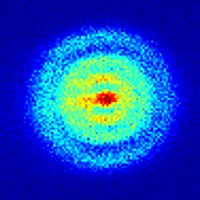
\includegraphics[scale=3.0]{Images/art_quantum.jpg}
	\caption{The first photograph of a Hydrogen atom was captured by an ultra sensitive camera in 2013. One can actually see the probability distribution $|\Psi(\bs{r})|^2$ with the naked eye. Published in Phys. rev. lett. 110, 213001 (2013), \textit{Hydrogen atoms under magnification}. \cite{stodolna_hydrogen_2013}}
\end{figure}

In the early 20th century, some scientists claimed that there were nothing new to be discovered in physics. They though that the deviation from experimental results were caused by uncertainties in the measurements and that the theory was complete. \cite{weisstein_kelvin_2007} They could not be more wrong.

Just a few years later in 1905, Albert Einstein published a paper advancing Max Planck's hypothesis that the energy of light is carried in discrete quantized packets to explain the photoelectric effect. This was a vital step in the development of quantum mechanics. \footnote{The same year, Einstein presented his special theory of relativity, followed by the general theory of relativity in 1915. This theory superseded a 200-year-old theory of mechanics created primarily by Isaac Newton.} The years after this discovery, immense efforts were placed on completing the theory, and contributions from an array of scientists over a period of more than 20 years were necessary to complete what today is known as the quantum theory. 

Key people include Niels Bohr, who developed a model to explain the spectral lines in atoms, Max Born who suggested the now-standard interpretation of the probability density function, Werner Heisenberg who formulated the matrix mechanics of quantum mechanics, Erwin Schrödinger who formulated the wave mechanics of quantum mechanics and Paul Dirac who contributed to complete the theory. We will meet them again and again throughout this thesis.

In 1929, Paul Dirac formulated something similar to what the scientists had claimed in the early 20th century, but apparently more correctly. \cite{dirac_paul_adrien_maurice_quantum_1929}

\newpage
\section{Preliminary quantum physics} \label{sec:elementary}
In this section we will present the fundamentals of the quantum theory, which will make up the framework of this project. The theory is based on David Griffith's incredible textbook, \textit{Introduction to Quantum Mechanics}, where the reader is relegated for further information.

Before we get started, we make a few assumptions in order to simplify our problem. The most important ones are specified below with an explanation why they are valid.

\begin{itemize}
	\item \textbf{Point-like particles:} First, all particles involved will be assumed to be point-like, i.e, they lack spatial extension. For electrons this makes sense, since they, as far as we know, do not extent. The assumption is also applied on the nucleus in atomic systems, but it still makes sense since the distance from the nucleus to the electrons is known to be much larger than the nucleus extent.
	
	\item \textbf{Non-relativistic spacetime:}  Second, we operate in the non-relativistic spacetime, which is an extremely good approximation as long as we do not approach the speed of light and we do not involve strong forces. Applying classical physics, we can find that the speed of the electron in a hydrogen atom is about 1\% of the speed of light, and even though the electrons get higher speed in heavier atoms, we do not need to worry about it as we will stick to the lighter atoms. The forces acting are the weak Coulomb forces. In the quantum dots, this assumption hold even for large systems.
	
	\item For specific systems we might make new assumptions and approximations. For instance, for atomic systems we will assume that the nucleus is at rest. Those approximations will be discussed consecutively. 
\end{itemize}

\subsection{The Schrödinger equation} \label{subsec:schrodinger}
In this work we will focus on solving the time-independent non-relativistic Schrödinger equation, which gives the energy eigenvalues of a system defined by a Hamiltonian $\hat{\mathcal{H}}$ and its eigenfunctions, $\Psi_n(\bs{r})$, which are the wave functions. $\bs{r}$ are the position coordinates of all the system's particles and $n$ characterizes the state. The equation reads
\begin{equation}
\label{eq:Energy}
 \hat{\mathcal{H}}\psin=\epsilon_n\psin
\end{equation}
where the Hamiltonian is operator of total energy. By analogy with the classical mechanics, this is given by
\begin{equation}
\hat{\mathcal{H}}=\hat{\mathcal{T}}+\hat{\mathcal{V}}
\end{equation}
with $\hat{\mathcal{T}}$ and $\hat{\mathcal{V}}$ as the kinetic and potential energy operators respectively. 

Again from classical mechanics, the kinetic energy for a moving particle of mass $m$ yields $T=p^2/2m$ where $p$ is the linear momentum, such that the kinetic energy operator can be represented as 
\begin{equation}
\hat{\mathcal{T}}=\frac{\hat{\mathcal{P}}^2}{2m}
\end{equation}
according to Ehrenfest's theorem. Further, the linear momentum operator is $\hat{\mathcal{P}}=-i\hbar\hat{\nabla}$ with $\hat{\nabla}$ as the differential operator and $\hbar$ as the reduced Planck's constant.

The potential energy can be split into an external part and an interaction part, where the latter is given by the Coulomb interaction. For two identical particles of charge $q$, the repulsive interaction gives the energy
\begin{equation}
V_{\text{int}} =k_e\frac{q^2}{r_{12}}
\end{equation}
where $r_{12}$ is the distance between the particles and $k_e$ is Coulomb's constant. The total Hamiltonian of a system of $N$ identical particles takes the form
\begin{equation}
\hat{\mathcal{H}}=-\sum_i^N\frac{\hbar^2}{2m}\nabla_i^2+\sum_i^{N}u_i + \sum_i^N\sum_{j>i}^Nk_e\frac{q^2}{r_{ij}}
\label{eq:ElectronicHamiltonian}
\end{equation}
which is the farthest we can go without specifying the external potential $u_i$. $r_{ij}$ is the relative distance between particle $i$ and $j$, defined by $r_{ij}\equiv|\bs{r}_i-\bs{r}_j|$.

Setting up equation \eqref{eq:Energy} with respect to the energies, we obtain an integral,
\begin{equation}
\epsilon_n=\frac{\int d\bs{r}\psinc\hat{\mathcal{H}}\psin}{\int d\bs{r}\psinc\psin},
\label{eq:energyintegral}
\end{equation}
which not necessarily is trivial to solve. As suggested by Max Born, we get the probability distribution function if we take the dot product between the complex conjugate wave function and the wave function itself,
\begin{equation}
P(\bs{r})=\psinc\psin=|\psin|^2,
\end{equation}
so the denominator is basically the integral over all the probabilities. If the wave function is normalized correctly, this should always give 1. 

\subsection{Statistical interpretation}
In equation \eqref{eq:energyintegral}, we found the expectation value of the energy using the Hamiltonian, which is the energy operator. However, this relation applies for an arbitrary operator $\mathcal{\hat{O}}$ related to an expectation value $\langle \mathcal{\hat{O}}\rangle$,
\begin{equation}
\langle \mathcal{O}\rangle=\frac{\int d\bs{r}\psinc\hat{\mathcal{O}}\psin}{\int d\bs{r}\psinc\psin}.
\label{eq:generalexp}
\end{equation}
As a consequence, there is always an uncertainty associated with a measurement in quantum physics, which means that we can only tell the probability of measuring something. The variance of measurements is given by
\begin{equation}
\sigma^2=\langle \mathcal{O}^2\rangle-\langle \mathcal{O}\rangle^2
\label{eq:variance}
\end{equation}
and if we take the square root of this we will get the standard deviation.
From this, a variety of mathematical inequalities follows, where Heisenberg's uncertainty principle is the most famous. It states that the more precisely the position of some particle is determined, the less precisely its momentum can be known, and is mathematically presented as
\begin{equation}
\sigma_x\sigma_p\geq\frac{\hbar}{2}
\end{equation}
where $\sigma_x$ is the standard deviation of the position and $\sigma_p$ is the standard deviation of the momentum. This standard deviation gives the statistical uncertainties. 

Before we end this section, we will introduce the Dirac formalism, which is a elegant and efficient way of describing quantum states. For instance, equation \eqref{eq:generalexp} can, using Dirac formalism, be written as
\begin{equation}
\langle \mathcal{O}\rangle=\frac{\mel{\Psi}{\mathcal{\hat{O}}}{\Psi}}{\braket{\Psi}{\Psi}}
\end{equation}
where $\bra{\Psi}$ is called the \textit{bra} and $\ket{\Psi}$ is called the \textit{ket}. For that reason, the formalism is also called braket formalism. 

Often, the inner product in the denominator is assumed to be 1, such that the expectation value can be simplified to
\begin{equation}
\langle \mathcal{O}\rangle=\mel{\Psi}{\mathcal{\hat{O}}}{\Psi},
\end{equation}
which we will henceforth assume. More information about the Dirac formalism can be found in Appendix A. 

\subsection{The variational principle}
In the equations above, the presented wave functions are assumed to be the exact eigenfunctions of the Hamiltonian. But often we do not know the exact wave functions, and we need to guess what the wave functions might be. In those cases we make use of the Rayleigh-Ritz variational principle or just the variational principle, which states that only the exact ground state wave function is able to give the ground state energy. All other wave functions that fulfill the required properties (see section \ref{sec:wavefunction}) give higher energies, and mathematically we can express the statement as
\begin{equation}
\epsilon_0\leq\mel{\Psi_T}{\hat{\mathcal{H}}}{\Psi_T}.
\label{eq:variationalprinciple}
\end{equation}

Variational Monte-Carlo is a quantum many-body method based on (and named after) the variational principle, where we vary the trial wave function in order to obtain the lowest energy. It will be detailed in chaper \eqref{chp:methods}.

\subsection{Quantum numbers}
Unlike in the classical mechanics, all the observable in quantum mechanics are discrete or \textit{quantized}, which means that the $n$ associated with $\varepsilon_n$ above cannot take any number. In fact, $n$ can only take positive integers, and is named the principal quantum number.

\subsubsection*{Principal}
The \textbf{principal} quantum number describes the electron shell, and can take the numbers $n\in[1,2,3,\hdots)$. As $n$ increases, the electron excites to a higher shell such that also the energy increases. In general, $\varepsilon_1<\varepsilon_2<\varepsilon_3\hdots$ as long as all other quantum numbers are fixed. The electron shells can again be split up in subshells, requiring more quantum numbers.

\subsubsection*{Angular}
An electron shell can possibly have more than one subshell, described by the \textbf{angular} quantum number $l$. $l$ can take the values $0,1,\hdots n-1$, such that the degeneracy of subshells in a shell is simply $n$. In atoms, the angular quantum number describes the shape of the shell, where $l=0$ gives a spherical shape, $l=1$ gives a polar shape while $l=2$ gives a cloverleaf shape. 

\subsubsection*{Magnetic}
We also have a \textbf{magnetic} quantum number $m_l$, which has the range $-l,-l+1,\hdots,l-1,l$. If $l$ describes the shape of a shell, $m_l$ specifies its orientation in space. This quantum number was first observed under presence of a magnetic field, hence the name.

\subsubsection*{Spin}
The \textbf{spin} quantum number $s$ gives the spin of a particle, which can just be seen as a particle's property. Particles are often divided in two groups dependent on the spin because of their different behavior: \textbf{bosons} have integer spin, while \textbf{fermions} have half-integer spin. Electrons and protons have spin $s=1/2$, which makes them fermions.

\subsubsection*{Spin projection}
The last number we will discuss is the \textbf{spin projection} quantum number $m_s$. It has the range $-s,-s+1,\hdots,s-1,s$, and is therefore related to the spin quantum number in the same way as $m_l$ is related to the angular quantum number. Electrons can for that reason take the values $m_s=+1/2$ or $m_s=-1/2$, such that there are two groups of electrons. The consequences will be discussed in the section \eqref{sec:wavefunction}.

\subsection{The Virial Theorem} \label{sec:virial}
The virial theorem relates the kinetic energy to the potential energy, and makes it possible to find the average kinetic energy even for complex systems. The classical statement of the theorem was formulated during the 19th century and named by Rudolf Clausius in 1870, \cite{clausius_xvi._1870}, and is in the most general form given by 
\begin{equation}
\langle\mathcal{T}\rangle=-\frac{1}{2}\sum_{i=1}^N\langle\bs{F}_i\cdot\bs{r}_i\rangle
\end{equation}
where $\bs{F}_k$ represents the force on particle $i$ at position $\bs{r}_i$. If we further assume that all the sources of potential are on the form $\mathcal{V}_i=ar^{n_i}$, we can use the relation $\bs{F}_i=-\nabla \mathcal{V}_i$ to express the virial theorem in a simpler fashion
\begin{equation}
2\langle \mathcal{T} \rangle = \sum_{i}n_i\langle \mathcal{V}_{i} \rangle.
\end{equation}
Vladimir Fock proved that this holds for quantum mechanics in 1930. \cite{fock_bemerkung_1930} The assumption raised above holds for our situation as the interaction energy does as $r^{-1}$. We will also later see that the potential used in quantum dots goes as $r^2$ and the potential used in atoms goes as $r^{-1}$ as well.

The expectation value is in principle the time average of the operator. However, if the ergodic hypothesis hold for the system, an ensemble average can also be taken. Ergodicity means that the ensemble average is equal to the time average. \cite{flyvbjerg_error_1989}


\iffalse
\begin{equation}
2\langle \mathcal{\hat{T}} \rangle = 2\langle \mathcal{\hat{V}_{\text{ext}}} \rangle - \langle \mathcal{\hat{V}_{\text{int}}} \rangle
\end{equation}
\fi

\iffalse
\subsubsection*{Angular Momentum and Spin}
Relation between the angular and spin quantum number

(One last analogy with the classical mechanics)

If we again go back to the classical mechanics, the angular momentum $\bs{L}_r=\bs{R}\cross\bs{p}$ around an axis at distance $|\bs{R}|$ from the mass center and the angular momentum $\bs{L}_c=I\bs{\omega}$ around its own mass center is a conserved quantity,
\begin{equation}
\bs{L}_{net} = \bs{L}_r+\bs{L}_c.
\end{equation}
Since the net angular momentum $\bs{L}_{new}$ is just a sum over the angular momentum of all points in a continua around the rotational axis given by the definition of $\bs{L}_r$, both of them are actually the same thing.

In quantum mechanics we have again an analogy, where we define a \textbf{spin} $s$ which describes a particles rotation around its own mass center and a \textbf{angular momentum} $l$ which describes a particles rotation around an external rotational axis. Like in classical physics, the total spin $S$ and the total angular momentum $L$ is a conserved quantity,
\begin{equation}
J=L+S,
\end{equation}
but the transition from $L$ to $S$ is rare compared to the transition from $L_c$ to $L_r$. Spin-orbit coupling. Azimuthal. Quantized.

We will summary all the quantum numbers through a table. 

\subsubsection*{Hund's Rules}
Hund's rules define the filling order of electron structure shells with respect to the ground state energy. 
\fi

\subsection{Postulates of Quantum Mechanics}
The quantum theory is built on six fundamental postulates, which should always hold. Some of them are already described, but here we present the complete list. Without mentioning them our section on quantum theory would be incomplete. The postulates write:

\begin{enumerate}
\item \textit{"The state of a quantum mechanical system is completely specified by the wave function $\Psi(\bs{r},t)$."}

\item \textit{"To every observable in classical mechanics, there corresponds a linear, Hermitian operator in quantum mechanics."}

\item \textit{"In any measurement of the observable associated with an operator $\hat{\mathcal{O}}$, the only values that will ever be observed are the eigenvalues $o$ which satisfy $\hat{\mathcal{O}}\Psi=o\Psi$."}

\item \textit{"The expectation value of the observable corresponding to operator $\hat{\mathcal{O}}$ is given by
$$\langle\mathcal{O}\rangle=\frac{\int d\tau\Psi^*\hat{\mathcal{O}}\Psi}{\int d\tau\Psi^*\Psi}.\textit{"}$$}

\item \textit{"The wave function evolves in time according to the time-dependent Schrödinger equation,
$$\hat{\mathcal{H}}\Psi(\bs{r},t)=i\hbar\frac{\partial\Psi}{\partial t}.\textit{"}$$}

\item \textit{"The total wavefunction must be antisymmetric with respect to the interchange of all coordinates of one fermion with those of another. Electronic spin must be included in this set of coordinates."} 
\end{enumerate}
The postulates are taken from \cite{sherrill_david_postulates_2003}.

Since we will be looking at stationary systems only, the time-independent Schrödinger equation and then postulate no.5 will not be utilized, but apart from that they all will play a significant role. 

\section{The trial wave function} \label{sec:wavefunction}
By the first postulate of quantum mechanics, the wave function contains all the information specifying the state of the system. This means that all observable in classical mechanics can also be measured from the wave function, which makes finding the wave function our main goal.

The trial wave function needs to meet some requirements in order to be used in the variational principle, and we thus need to make an educated guess on the wave function where the requirements are fulfilled. The requirements are the following:

\begin{enumerate}
	\item \textbf{Normalizability:} The wave function needs to be normalizable in order to be physical. The total probability should always be 1, and a wave function that cannot be normalized will not have a finite total probability. The consequence is that the wave function needs to converge to zero when the positions get large. 
	
	\item \textbf{Cusp condition:} The cusp condition (also called the Kato theorem) states that the wave function should have a cusp where the potential explodes. An example on this is when charged particles come close to each other. 
	
	\item \textbf{Symmetry and anti-symmetry:} The wave function needs to be either symmetric or anti-symmetric under exchange of two coordinates, dependent on whether the particles are fermions or bosons. This is the statement of the sixth postulate, which will be further explained in the next section.
\end{enumerate}

\subsection{Anti-symmetry and the Pauli principle} \label{subsubsec:symmetry}
Assume that we have a permutation operator $\hat{P}$ which exchanges two coordinates in the wave function,
\begin{equation}
\hat{P}(i\rightarrow j)\Psi_n(\bs{x}_1,\hdots,\bs{x}_i,\hdots,\bs{x}_j,\hdots,\bs{x}_M)=p\Psi_n(\bs{x}_1,\hdots,\bs{x}_j,\hdots,\bs{x}_i,\hdots,\bs{x}_M),
\end{equation}
where $p$ is just a factor which comes from the transformation. If we again apply the $\hat{P}$ operator, we should switch the same coordinates back, and we expect to end up with the initial wave function. For that reason, $p$ must be either +1 or -1. \footnote{Actually, in two-dimensional systems we have a third possibility which gives an \textit{anyon}. The theory on this was developed by J.M. Leinaas and J. Myrheim during the 1970's. \cite{leinaas_one_1977}}

The particles that have an antisymmetric (AS) wave function under exchange of two coordinates are called fermions, named after Enrico Fermi, and as discussed before they have half-integer spin. On the other hand, the particles that have a symmetric (S) wave function under exchange of two coordinates are called bosons, named after Satyendra Nath Bose, and have integer spin. 

It turns out that because of their anti-symmetric wave function, two identical fermions cannot be found at the same position at the same time, known as the Pauli principle. 

The probability of finding two identical particles at the same position at the same time should be zero due to the Pauli principle, so technically we need to set the wave function to zero if it happens. To deal with this, we introduce a so-called Slater determinant, which automatically sets the wave function to zero if the principle is not satisfied.

\subsection{Slater determinant} \label{subsec:slater}
For a system of many particles we can define a total wave function, which is a composition of all the single particle wave functions (SPF) and contains all the information about the system as the first postulate requires. For fermions, we need to combine the SPFs such that the Pauli principle is fulfilled at all times, which can be accomplished by a determinant. 

Consider a system of two identical fermions with SPFs $\phi_1$ and $\phi_2$ at positions $\boldsymbol{r}_1$ and $\boldsymbol{r}_2$ respectively. The way we define the wavefunction of the system is then
\begin{equation}
\Psi_T(\bs{r}_1,\bs{r}_2)=
\begin{vmatrix}
\phi_1(\boldsymbol{r}_1) & \phi_2(\boldsymbol{r}_1)\\
\phi_1(\boldsymbol{r}_2) & \phi_2(\boldsymbol{r}_2)
\end{vmatrix}
=\phi_1(\boldsymbol{r}_1)\phi_2(\boldsymbol{r}_2)-\phi_2(\boldsymbol{r}_1)\phi_1(\boldsymbol{r}_2),
\end{equation}
which is set to zero if the particles are at the same position. The determinant yields the same no matter the size of the system.

The Slater determinant is just a wave function ansatz to satisfy the Pauli principle, and we therefore need to denote it as the trial wave function. Additionally, the Slater determinant above contains the radial part only, because the single particle functions are the radial part by convention. For a general Slater determinant of $N$ particles, the spin part needs to be included as well, giving 
\begin{equation}
\Psi_T(\bs{r})=
\begin{vmatrix}
\psi_1(\boldsymbol{r}_1) & \psi_2(\boldsymbol{r}_1) & \hdots & \psi_N(\boldsymbol{r}_1)\\
\psi_1(\boldsymbol{r}_2) & \psi_2(\boldsymbol{r}_2) & \hdots & \psi_N(\boldsymbol{r}_2)\\
\vdots & \vdots & \ddots & \vdots \\
\psi_1(\boldsymbol{r}_N) & \psi_2(\boldsymbol{r}_N) & \hdots & \psi_N(\boldsymbol{r}_N)
\end{vmatrix}
\end{equation}
where the $\psi$'s are the true single particle wave functions, which are the tensor products 
\begin{equation}
\psi=\phi\otimes\xi
\end{equation}
with $\xi$ as the spin part. In the next section, we will proceed further and show how the spin part can be factorized out of a general Slater determinant.

For bosonic systems, one can correspondingly construct a Slater permanent. The permanent of a matrix is similar to the determinant, but all negative signs are replaced by positive signs. 

\subsection{Splitting up the Slater determinant} \label{subsec:electronsystem}
A determinant is relative computational expensive, and as the number of particles increases, it will certainly give us some problems. Fortunately, the Slater determinant can be split up when the particles have different spin, which is often hugely beneficial. Not only does the dimensions of the determinant reduce, but this makes it also possible to factorize out the spin part.

In this work, we will study fermions of spin $\sigma=\pm 1/2$ only, and we will therefore do the splitting for this specific case. However, this case is very important since both electrons and protons among others are spin-1/2 particles. The particles with $\sigma=+1/2=\uparrow$ will be denoted as the spin-up particles, and the particles with $\sigma=-1/2=\downarrow$ will be denoted as the spin-down particles. For simplicity, we will assume that the first coordinates $\bs{r}_1,\hdots\bs{r}_{N_{\uparrow}}$ are the coordinates of the spin-up particles and the coordinates $\bs{r}_{N_{\uparrow}+1},\hdots\bs{r}_N$ are associated with the spin-down particles. $N_{\uparrow}$ is the number of spin-up particles and $N_{\downarrow}$ is the number of spin-down particles. The Slater determinant can then be written as
\begin{equation*}
\Psi(\boldsymbol{r})=
\begin{vmatrix}
\phi_1(\boldsymbol{r}_1)\xi_{\uparrow}(\uparrow) & \hdots & \phi_{N_{\uparrow}}(\boldsymbol{r}_1)\xi_{\uparrow}(\uparrow) & \phi_{N_{\uparrow}+1}(\boldsymbol{r}_1)\xi_{\downarrow}(\uparrow) & \hdots & \phi_{N}(\boldsymbol{r}_1)\xi_{\downarrow}(\uparrow)\\
\vdots & & \vdots & \vdots & & \vdots \\
\phi_1(\boldsymbol{r}_{N_{\uparrow}})\xi_{\uparrow}(\uparrow) & \hdots & \phi_{N_{\uparrow}}(\boldsymbol{r}_{N_{\uparrow}})\xi_{\uparrow}(\uparrow) & \phi_{N_{\uparrow}+1}(\boldsymbol{r}_{N_{\uparrow}})\xi_{\downarrow}(\uparrow) & \hdots & \phi_{N}(\boldsymbol{r}_{N_{\uparrow}})\xi_{\downarrow}(\uparrow)\\
\phi_1(\boldsymbol{r}_{N_{\uparrow}+1})\xi_{\uparrow}(\downarrow) & \hdots & \phi_{N_{\uparrow}}(\boldsymbol{r}_{N_{\uparrow}+1})\xi_{\uparrow}(\downarrow) & \phi_{N_{\uparrow}+1}(\boldsymbol{r}_{N_{\uparrow}+1})\xi_{\downarrow}(\downarrow) & \hdots & \phi_{N}(\boldsymbol{r}_{N_{\uparrow}+1})\xi_{\downarrow}(\downarrow)\\
\vdots & & \vdots & \vdots & & \vdots \\
\phi_1(\boldsymbol{r}_N)\xi_{\uparrow}(\downarrow) & \hdots & \phi_{N_{\uparrow}}(\boldsymbol{r}_N)\xi_{\uparrow}(\downarrow) & \phi_{N_{\uparrow}+1}(\boldsymbol{r}_N)\xi_{\downarrow}(\downarrow) & \hdots & \phi_{N}(\boldsymbol{r}_N)\xi_{\downarrow}(\downarrow)\\
\end{vmatrix},
\end{equation*}
where spin-up wave functions require spin-up particles and vice versa. For that reason, half of the elements become zero and the determinant can be further expressed as
\begin{equation*}
\Psi(\boldsymbol{r})=
\begin{vmatrix}
\phi_1(\boldsymbol{r}_1)\xi_{\uparrow}(\uparrow) & \hdots & \phi_{N_{\uparrow}}(\boldsymbol{r}_1)\xi_{\uparrow}(\uparrow) & 0 & \hdots & 0\\
\vdots & & \vdots & \vdots & & \vdots \\
\phi_1(\boldsymbol{r}_{N_{\uparrow}})\xi_{\uparrow}(\uparrow) & \hdots & \phi_{N_{\uparrow}}(\boldsymbol{r}_{N_{\uparrow}})\xi_{\uparrow}(\uparrow) & 0 & \hdots & 0\\
0 & \hdots & 0 & \phi_{N_{\uparrow}+1}(\boldsymbol{r}_{N_{\uparrow}+1})\xi_{\downarrow}(\downarrow) & \hdots & \phi_{N}(\boldsymbol{r}_{N_{\uparrow}+1})\xi_{\downarrow}(\downarrow)\\
\vdots & & \vdots & \vdots & & \vdots \\
0 & \hdots & 0 & \phi_{N_{\uparrow}+1}(\boldsymbol{r}_N)\xi_{\downarrow}(\downarrow) & \hdots & \phi_{N}(\boldsymbol{r}_N)\xi_{\downarrow}(\downarrow)\\
\end{vmatrix}.
\end{equation*}
This determinant can by definition be split up in a product of two determinants,
\begin{equation}
\Psi(\boldsymbol{r})=|\hat{D}_{\uparrow}|\cdot |\hat{D}_{\downarrow}|
\end{equation}
where $\hat{D}_{\uparrow}$ is the matrix containing all spin-up states and $\hat{D}_{\downarrow}$ is the matrix containing all spin-down states. Since all elements in the respective matrices contain the same spin function, it can be factorized out and omitted in the future study since the energy is independent of spin.

It is also worth to notice that the size of the spin-up determinant is determined by the number of spin-up particles, and it is similar for the spin-down determinant. This means that the we can change the total spin $S$ by adjusting the relative sizes of the determinants.

This section was heavily inspired by D.Nissenbaum's dissertation, see appendix I in \cite{nissenbaum_stochastic_2008}.

\subsection{Basis set} \label{subsec:basisset}
To go further, we need to define a basis set, $\{\phi_1(\bs{r}),\phi_2(\bs{r}),\hdots\phi_N(\bs{r})\}$ which should be chosen carefully based on the system. For a few systems, we know the exact basis of the non-interacting case, and it is thus a natural basis to use in the Slater determinant. For other systems, the choice of basis might depend on the situation, where we typically need to weigh computational time against accuracy. Concrete examples on both cases will be presented in chapter \eqref{chp:systems}.

Often, one will see that the basis is optimized by the Hartree-Fock method. Using this basis in a single Slater determinant, we obtain the Hartree-Fock energy which sometimes is quite accurate. To get an even better energy estimate, we need to add more Slater determinants, which is the task of the post Hartree-Fock methods. More about this in chapter (\ref{chp:methods},\ref{chp:othermethods}).

\subsection{Jastrow factors} \label{subsubsec:jastrow}
From electrostatics we know that identical, charged particles will repel each other. This means that the probability of finding two particles close to each other should be low, which needs to be baked into the wave function. One way to do this is to simply multiply the wave function with the distance between the particles; the smaller distance the lower probability. However, since we are going to work in the logarithmic space, dealing with exponential function will be much easier. This is the main idea behind the simple Jastrow factor.

\subsubsection{Simple Jastrow}
The simple Jastrow factor is just an exponential function with the sum over all particle distances. In addition, each distance $r_{ij}$ is weighted by a parameter $\beta_{ij}$, and the factor becomes
\begin{equation}
J(\bs{r}; \bs{\beta}) = \exp\left(\sum_{i=1}^N\sum_{j>i}^N{\beta_{ij}r_{ij}}\right).
\label{eq:SimpleJastrow}
\end{equation}
All the $\beta_{ij}$ are free variational parameters, which are expected to be symmetric since the distance matrix is symmetric.

One problem with this Jastrow factor, is that it does not create the cusp around each particle correctly. Basically, the Jastrow factor increases faster than it should when a particle is moved away from another. To solve this, we need to introduce a more complex Jastrow factor, the Padé-Jastrow.

\subsubsection{Padé-Jastrow}
The Padé-Jastrow factor is closely related to the simple Jastrow above, but a denominator is added to make the cusp correctly. It reads
\begin{equation}
J(\bs{r};\beta) = \exp\bigg(\sum_{i=1}^N\sum_{j>i}^N\frac{a_{ij}r_{ij}}{1+\beta r_{ij}}\bigg).
\label{eq:PadeJastrow}
\end{equation}
where $\beta$ is a variational parameter. In addition, the fractions are multiplied with constants $a_{ij}$ which depend on the particles $i$ and $j$ in the following way:
\begin{equation}
\label{eq:ajastrow}
a_{ij}=
\begin{cases} 
e^2/(D+1) & \text{if $i,j$ are particles of same spin} \\
e^2/(D-1) & \text{if $i,j$ are particles of opposite spin},
\end{cases}
\end{equation}
for dimensions $D\in[2,3]$ where $e$ is the elementary charge. We will later use natural and atomic units, and set $e=1$, which for two dimensions gives $a_{ij}=1/3$ (same spin) or $a_{ij}=1$ (opposite spin) and for three dimensions $a_{ij}=1/4$ (same spin) and $a_{ij}=1/2$ (opposite spin). \cite{hogberget_quantum_2013,mariadason_quantum_2018}

This Jastrow factor is known to give accurate results for fermions and bosons because it gives the correct cusp condition, and it is the one we gonna use in the standard variational Monte-Carlo simulations.

\section{Electron density}
In quantum many-body computations, the electron density is frequently calculated, and there are several reasons for that. Firstly, the electron density can be found experimentally, such that the calculations can be benchmarked. Secondly, the electron density is very informative, since information about all particles can be gathered in one plot.

The $P$-body electron density can be found by integrating over all particles but $P$, 
\begin{equation}
\label{eq:electron_density}
\rho_i(\bs{r})=\int_{-\infty}^{\infty}d\bs{r}_P\hdots d\bs{r}_N |\Psi(\bs{r}_1,\hdots \bs{r}_N)|^2.
\end{equation}
where $P<N$.

\subsection{One-body Density}
The one-body density is the most applied electron density, and is sometimes simply referred to as the electron density. For the two particle case, the one-body density gives the probability of finding one particle at a relative distance $r$ to the other. For more particles, the one-body density gives the probability of finding the mass center of the remaining particles at a relative distance $r$ from one of the particles.

The one-body density integral can be solved by Monte-Carlo integration. We then divide the space into bins of equal sizes at different radii and count the number of particles in each bin throughout the sampling. In practice, one often divide the space into bins where the radii are uniformly distributed, i.e, $r_i=i\cdot r_0$, see figure \eqref{fig:onebody}. In that case, one needs to divide the number of particles in each bin by its volume afterwards in order to get a correct distribution. In two dimensions, the area of bin $i$ is
\begin{equation}
A_i=(2i+1)\pi d^2
\end{equation}
and in three dimensions the volume of bin $i$ is
\begin{equation}
V_i=4(i(i+1)+1/3)\pi d^3.
\end{equation}
where $d$ is the radial width of a bin. 

\begin{figure}
	\centering
	\label{fig:onebody}
	\begin{tikzpicture}[scale=0.50, thick, dot/.style={shape=circle,inner sep=+0pt, minimum size=+2pt, fill, label={#1}}]
   \coordinate[dot={$\bs{r}_i$}] (ri) at (4.8,4);
   \coordinate[dot] (center) at (1,4);
   \coordinate[] (point) at (1,7);

   \foreach \cnt[count=\Cnt from 0] in {0, .5, 1, 1.5, 2}
     \node[
     draw, 
     label={[inner sep=+7pt] below:${\Cnt}$}
     ] 
     at (center) [circle through=($(center)!\cnt!(point)$)] {};
   \node at (15,4) {
   \begin{tabular}{|c|c|c|c|c|} \hline
   $\phantom{+1}$ & $\phantom{+1}$ & $+1$ & $\phantom{+1}$ & $\phantom{+1}$ \\ \hline
   \multicolumn{1}{c}{0} & \multicolumn{1}{c}{1} & \multicolumn{1}{c}{2} & \multicolumn{1}{c}{3} & \multicolumn{1}{c}{4}
   \end{tabular}};

	\draw[color0,ultra thick,->] (ri) to [out=270,in=270] (15,3);
	\draw[<->, color1] (-3.5,4) -- (-2,4) node[midway,below,color1] {$\Delta r$};
\end{tikzpicture}
	\caption{This figure is meant to illustrate how the one-body density is calculated using Monte-Carlo integration. One divides the space into $n$ bins (here 5), and count the number of particles in each bin throughout the sampling. Afterwards, the bins need to be normalized.}
\end{figure}

\begin{figure}
	\centering
	\label{fig:twobody}
	\begin{tikzpicture}[scale=0.50, thick, dot/.style={shape=circle,inner sep=+0pt, minimum size=+2pt, fill, label={#1}}]
\coordinate[dot={$\bs{r}_i$}] (ri) at (4.8,4);
\coordinate[dot={$\bs{r}_j$}] (rj) at (2,5.5);
\coordinate[dot] (center) at (1,4);
\coordinate[] (point) at (1,7);

\foreach \cnt[count=\Cnt from 0] in {0, .5, 1, 1.5, 2}
\node[
draw, 
label={[inner sep=+7pt] below:${\Cnt}$}
] 
at (center) [circle through=($(center)!\cnt!(point)$)] {};
\node at (15,4) {
	\begin{tabular}{c|c|c|c|c|c|} \cline{2-6}
	4 &$\phantom{+1}$ & $\phantom{+1}$ & $\phantom{+1}$ & $\phantom{+1}$ & $\phantom{+1}$ \\ \cline{2-6}
	3 &$\phantom{+1}$ & $\phantom{+1}$ & $\phantom{+1}$ & $\phantom{+1}$ & $\phantom{+1}$ \\ \cline{2-6}
	2 &$\phantom{+1}$ & $\phantom{+1}$ & $\phantom{+1}$ & $\phantom{+1}$ & $\phantom{+1}$ \\ \cline{2-6}
	1 &$\phantom{+1}$ & $\phantom{+1}$ & $+1$ & $\phantom{+1}$ & $\phantom{+1}$ \\ \cline{2-6}
	0 &$\phantom{+1}$ & $\phantom{+1}$ &$\phantom{+1}$ & $\phantom{+1}$ & $\phantom{+1}$ \\ \cline{2-6}
	\multicolumn{1}{c}{}&\multicolumn{1}{c}{0} & \multicolumn{1}{c}{1} & \multicolumn{1}{c}{2} & \multicolumn{1}{c}{3} & \multicolumn{1}{c}{4}
	\end{tabular}};

	\draw[red,->] (ri) to [out=270,in=270] (15.7,1);
	\draw[red,->] (rj) to [out=30,in=180] (9.5,3.5);
\end{tikzpicture}
	\caption{This figure is meant to illustrate how the two-body density is calculated using Monte-Carlo integration. One divides the space into $n$ bins (here 5), and store the position of a pair of particles in a matrix throughout the sampling. Afterwards, the bins need to be normalized.}
\end{figure}

\subsection{Two-body Density}
The two-body density describes...

For the one-body density, we integrate over all the particles but one, which corresponds to counting number of particles in each bin when doing Monte-Carlo integration. For the two-body density, we integrate over all particles but a \textit{particle pair}, which means that we need to find the position of each particle pair in order to solve the integral by Monte-Carlo integration. See figure \eqref{fig:twobody} for an illustration of this Monte-Carlo integration.

\subsection{Wigner Crystals} \label{sec:wigner}
A Wigner crystal is a solid phase where electrons form triangular lattices to minimize the potential energy. The phenomenon occurs only when the potential energy dominates the kinetic energy, since the electrons then are almost "at rest". 

To minimize the potential energy, the distances between the electrons should be maximized. To achieve this, the electrons form the triangular lattice shape, not so unlike Norwegians on the metro trying to maximize the distance to anyone else. For that reason, the electron density should approach discrete radial values, and the phenomenon should be observable in one-body density plots.



